\Variant{29.12.2025}
\QQ{1}{$156$ sonining natural böluvçilari yiğindisini toping.
\Opts{$98$}{$392$}{$398$}{$362$}}
\QQ{2}{Hisoblang:
\[\frac{2^4+2^2+1}{2^7-2}+\frac{3^4+3^2+1}{3^7-3}+\frac{4^4+4^2+1}{4^7-4}\]
\Opts{$\dfrac1{40}$}{$\dfrac9{40}$}{$1$}{$\dfrac7{40}$}}
\QQ{3}{Usta bir işni $4$ kunda, şogirdi esa $12$ kunda bajaradi. Usta va şogird birgalikda işning bir qismini $1$ kunda bajardi, qolgan işni esa şogird tugatdi. Jami iş neça kunda bajarildi?
\Opts{$9$}{$7$}{$10$}{$8$}}
\QQ{4}{Palto narxi $1\,200\,000$ edi. Birinçi marta narxini $40\%$ ga, keyin $10\%$ ga kamaytirildi. Paltoning hozirgi narxini toping.
\Opts{$1\,512\,000$}{$648\,000$}{$1\,560\,000$}{$1\,600\,000$}}
\QQ{5}{$1^3+2^3+3^3+\dots+59^3$ ifoda quyidagi qaysi songa qoldiqsiz bölinadi?
\Opts{$40$}{$60$}{$72$}{$48$}}
\QQ{6}{Hisoblang: $\sqrt{4^9+6^{10}+9^{10}}$
\Opts{$2^9+3^8$}{$2^3+3^5$}{$2^9+3^{10}$}{$5^{19}$}}
\QQ{7}{Agar $x=\dfrac{9-\sqrt{80}}2$ bölsa, $\sqrt{x^2+18x+81}+\sqrt{x^2-8\sqrt5x+80}$ ni hisoblang.
\Opts{$18+8\sqrt5$}{$18-8\sqrt5$}{$9-4\sqrt5$}{$9+4\sqrt5$}}
\QQ{8}{Arifmetik progressiyada $a_{20}+a_{17}=35$ va $a_{21}\cdot a_{16}=150$ bölsa, $a_2$ ni toping.
\Opts{$105$ yoki $-65$}{$100$ yoki $-65$}{$100$ yoki $70$}{$105$ yoki $-70$}}
\QQ{9}{$(a_n)$ arifmetik progressiya va $(b_n)$ geometrik progressiya hadlari. Agar $b_1+b_2+b_3=65$ va $b_2>b_1$, $b_1-a_1=1$, $b_2-a_2=8$, $b_3-a_3=35$, $b_1+b_2+b_3+\dots+b_n=200$ bölsa, $n$ ni toping.
\Opts{$4$}{$6$}{$8$}{$5$}}
\QQ{10}{Ifodani soddalaştiring:
\[\frac{a^{-6}+a^{-4}+a^{-2}}{a^6+a^4+a^2}\]
\Opts{$a^{-8}$}{$a^{-6}$}{$a^6$}{$a^8$}}
\QQ{11}{Agar $a+b=x$, $ab=y$ bölsa, $ab^3+a^3b+a^2+b^2+5ab+2a^2b^2$ ni $x$ va $y$ orqali ifodalang.
\Opts{$xy^2+x^2+3y$}{$xy^2+y^2+2y$}{$yx^2+y^2+3y$}{$yx^2+x^2+3y$}}
\QQ{12}{Ifodani soddalaştiring:
\[\frac{2\cos^2a}{\tg2a+\sin2a}\]
\Opts{$\ctg a$}{$\ctg2a$}{$\tg2a$}{$\tg a$}}
\QQ{13}{Tengsizlikni yeçing:
\[\sqrt{2\sin x}\le1\]
\Opts{$[2\pi k;\,\pi+2\pi k],\ k\in\mathbb Z$}{$\left[\pi k;\,\dfrac\pi6+\pi k\right]\cup\left[\dfrac{5\pi}6+\pi k;\,\pi+\pi k\right],\ k\in\mathbb Z$}{$\left[2\pi k;\,\dfrac\pi6+2\pi k\right]\cup\left[\dfrac{5\pi}6+2\pi k;\,\pi+2\pi k\right],\ k\in\mathbb Z$}{$\left[\dfrac\pi6+2\pi k;\,\pi+2\pi k\right]\cup\left[\dfrac{5\pi}6+2\pi k;\,\pi+2\pi k\right],\ k\in\mathbb Z$}}
\QQ{14}{Tenglamaning haqiqiy ildizlari köpaytmasini toping:
\[\left(\sqrt[4]{17-12\sqrt2}\right)^x+\left(\sqrt[4]{17+12\sqrt2}\right)^x=6\]
\Opts{$8$}{$2$}{$-8$}{$-4$}}
\QQ{15}{Tenglama neçta haqiqiy ildizga ega?
\[\frac{2\ln2-\ln5+\ln(2x+3)}{\ln x+\ln(x+3)}=1\]
\Opts{$1$ ta}{$2$ ta}{$3$ ta}{Haqiqiy yeçimga ega emas}}
\QQ{16}{$\begin{cases}3x-y=16,\\ x+2y=17\end{cases}$ tenglamalar sistemasi berilgan bölsa, $x+y$ ning qiymatini toping.
\Opts{$10$}{$12$}{$15$}{$11$}}
\QQ{17}{$x^4-3x^2+6x-3=0$ tenglama neçta haqiqiy ildizga ega?
\Opts{$1$ ta}{$2$ ta}{$4$ ta}{Haqiqiy yeçimga ega emas}}
\QQ{18}{Tengsizlikning neçta butun yeçimi bor?
\[\frac{x^2+5x+7}{x^2-5x+6}+1\le\frac9{3-x}\]
\Opts{$5$ ta}{$7$ ta}{$6$ ta}{Çeksiz köp}}
\QQ{19}{Neçta butun son tengsizlikning yeçimi böla olmaydi?
\[\sqrt{x^2-1}\ge x-2\]
\Opts{$1$ ta}{$2$ ta}{$3$ ta}{Çeksiz köp}}
\QQ{20}{$f(x)=x+\dfrac1x$ funksiya berilgan. Quyidagilardan qaysi biri töğri?
\Opts{$\bigl(f(x)\bigr)^3=x^3+\dfrac1{x^3}+f(x)$}{$\bigl(f(x)\bigr)^3=-3f(x)+x^3+\dfrac1{x^3}$}{$\bigl(f(x)\bigr)^3=x^3+\dfrac1{x^3}+3f\left(\dfrac1x\right)$}{$\bigl(f(x)\bigr)^3=x^3+3f\left(\dfrac1{x^3}\right)+\dfrac1{x^3}$}}
\QQ{21}{Aniq integralni hisoblang:
\[\int_0^{\pi}(x-1)\cos x\,dx\]
\Opts{$\pi-1$}{$\pi-2$}{$-2$}{$\pi+2$}}
\QQ{22}{$f(x)=\cos\left(kx^n\right)\cdot\lg\sqrt[n]{x+\sqrt{1+x^2}}$ funksiya berilgan. Agar $f'(2023)=2024$ bölsa, $f'(-2023)+2024$ ni hisoblang.
\Opts{$0$}{$2024$}{$4096$}{$4048$}}
\QQ{23}{Agar $f(x)=\dfrac3{\sqrt{x+1}}$ bölsa, $f^{-1}(2)$ ning qiymatini toping.
\Opts{$1\dfrac14$}{$2\dfrac14$}{$1\dfrac34$}{$2\dfrac34$}}
\QQ{24}{Rasmda berilgan maʼlumotlar asosida $x$ ning uzunligini toping.
\qfig{\begin{tikzpicture}[scale=0.85,font=\scriptsize]
\coordinate (O) at (0,0);
\coordinate (P0) at (-6,0); \coordinate (P1) at (-4.5,2.598); \coordinate (P2) at (-2.25,3.897); \coordinate (P3) at (0,3.897); \coordinate (P4) at (1.688,2.923); \coordinate (P5) at (2.531,1.461); \coordinate (P6) at (2.531,0);
\draw (O)--(P0)--(P1)--(P2)--(P3)--(P4)--(P5)--(P6)--cycle;
\foreach \p in {P1,P2,P3,P4,P5} \draw (O)--(\p);
\foreach \p/\q in {P1/P0,P2/P1,P3/P2,P4/P3,P5/P4,P6/P5} \draw ($(\p)!0.22cm!(\q)$) -- ($($(\p)!0.22cm!(\q)$)!1!-90:(\p)$) -- ($(\p)!0.22cm!(O)$);
\foreach \k in {0,...,5} {\draw ({180-30*\k}:0.55) arc ({180-30*\k}:{150-30*\k}:0.55); \node at ({165-30*\k}:0.95) {$30^\circ$};}
\node[below] at (-3,0) {\small$64$}; \node[below] at (O) {\small$O$}; \node[below] at (1.27,0) {\small$x$};
\end{tikzpicture}}
\Opts{$9\sqrt3$}{$27$}{$18\sqrt3$}{$18$}}
\QQ{25}{Rasmda tomoni $\sqrt3$ ga teng bölgan kvadrat berilgan. Kvadratning bir tomoni muntazam uçburçakning balandligiga teng bölsa, muntazam uçburçakning yuzini toping.
\qfig{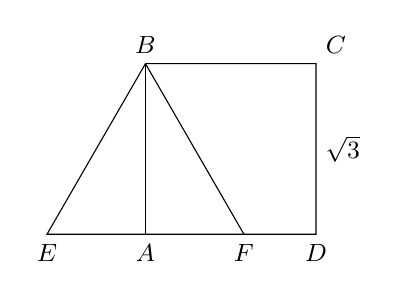
\begin{tikzpicture}[scale=1.25,font=\small]
\coordinate (A) at (0,0); \coordinate (B) at (0,1.732); \coordinate (C) at (1.732,1.732); \coordinate (D) at (1.732,0); \coordinate (E) at (-1,0); \coordinate (F) at (1,0);
\draw (E)--(D)--(C)--(B)--cycle; \draw (B)--(A); \draw (B)--(F);
\node[below] at (E) {$E$}; \node[below] at (A) {$A$}; \node[below] at (F) {$F$}; \node[below] at (D) {$D$};
\node[above] at (B) {$B$}; \node[above right] at (C) {$C$}; \node[right] at (1.732,0.866) {$\sqrt3$};
\end{tikzpicture}}
\Opts{$\dfrac{\sqrt3}2$}{$\sqrt3$}{$2$}{$3$}}
\QQ{26}{$ABC$ uçburçakning yuzi $96$ ga teng. Uçburçakning $AL$, $BD$, $CG'$ medianalaridan mos ravişda $F$, $E$, $K$ nuqtalar olingan va $AF=FL$, $BD=3BE$, $CG'=4CK$ bölsa, $FEK$ uçburçak yuzini toping.
\qfig{\begin{tikzpicture}[scale=1.15,font=\small]
\coordinate (A) at (0.000,0.000); \coordinate (B) at (1.470,3.170); \coordinate (C) at (3.900,0.000); \coordinate (L) at (2.685,1.585); \coordinate (D) at (1.950,0.000); \coordinate (G) at (0.735,1.585); \coordinate (F) at (1.343,0.792); \coordinate (E) at (1.630,2.113); \coordinate (K) at (3.109,0.396);
\fill[qfill] (F)--(E)--(K)--cycle;
\draw (A)--(B)--(C)--cycle; \draw (A)--(L); \draw (B)--(D); \draw (C)--(G); \draw (F)--(E)--(K)--cycle;
\node[below left] at (A) {$A$}; \node[above] at (B) {$B$}; \node[below right] at (C) {$C$}; \node[above right] at (L) {$L$};
\node[below] at (D) {$D$}; \node[above left] at (G) {$G'$}; \node[left] at (F) {$F$}; \node[above] at (E) {$E$}; \node[right] at (K) {$K$};
\end{tikzpicture}}
\Opts{$16$}{$19$}{$20$}{$24$}}
\QQ{27}{$ABCD$ töğri törtburçak berilgan. $AB=9$, $BC=11$ bölsa, böyalgan soha $EFGH$ yuzini toping.
\qfig{\begin{tikzpicture}[scale=0.27,font=\small]
\coordinate (A) at (0,0); \coordinate (B) at (9,0); \coordinate (C) at (9,11); \coordinate (D) at (0,11);
\coordinate (E) at (0,2); \coordinate (H) at (3,0); \coordinate (G) at (9,9); \coordinate (F) at (6,11);
\fill[qfill] (E)--(F)--(G)--(H)--cycle;
\draw (A)--(B)--(C)--(D)--cycle; \draw (E)--(F)--(G)--(H)--cycle;
\node[below left] at (A) {$A$}; \node[below right] at (B) {$B$}; \node[above right] at (C) {$C$}; \node[above left] at (D) {$D$};
\node[left] at (E) {$E$}; \node[above] at (F) {$F$}; \node[right] at (G) {$G$}; \node[below] at (H) {$H$};
\node[above] at (1.6,1) {$a$}; \node[right] at (6.2,4.3) {$3a$};
\end{tikzpicture}}
\Opts{$30$}{$39$}{$36$}{$45$}}
\QQ{28}{$ABCDE$ muntazam beşburçak berilgan. $DE$ tomoni $E$ tomonga davom ettirilib, unda $O$ nuqta olindi, $DO=8$. $G$ nuqta $AB$ tomonning örtasi bölib, $OG$ kesma $EA$ tomonni $F$ nuqtada kesib ötadi va $\angle OFE=45^\circ$. $H$ nuqta $BC$ tomonning örtasi. $EH$ ning uzunligini toping.
\qfig{\begin{tikzpicture}[scale=1.25,font=\small]
\coordinate (D) at (0.000,1.500); \coordinate (C) at (1.427,0.464); \coordinate (B) at (0.882,-1.214); \coordinate (A) at (-0.882,-1.214); \coordinate (E) at (-1.427,0.464); \coordinate (G) at (0.000,-1.214); \coordinate (H) at (1.154,-0.375); \coordinate (O) at (-2.195,-0.095); \coordinate (F) at (-1.057,-0.675);
\draw (A)--(B)--(C)--(D)--(E)--cycle; \draw (D)--(O)--(G); \draw (D)--(G); \draw (E)--(H);
\node[below] at (A) {$A$}; \node[below] at (B) {$B$}; \node[right] at (C) {$C$}; \node[above] at (D) {$D$}; \node[above left] at (E) {$E$};
\node[below] at (G) {$G$}; \node[right] at (H) {$H$}; \node[left] at (O) {$O$}; \node[below left] at (F) {$F$};
\node at ($(F)+(-25:0.33)$) {\scriptsize$45^\circ$};
\end{tikzpicture}}
\Opts{$8$}{$16$}{$8\sqrt2$}{$15$}}
\QQ{29}{$\vec a$, $\vec b$, $\vec c$ birlik vektorlarning ixtiyoriy ikkitasi orasidagi burçak $60^\circ$ ga teng. $\vec a$ va $\vec b+\vec c$ vektorlar orasidagi burçak kosinusini toping.
\Opts{$\dfrac{\sqrt2}2$}{$\dfrac1{\sqrt3}$}{$\dfrac{\sqrt3}2$}{$\dfrac{\sqrt3}4$}}
\QQ{30}{$\alpha$ va $\beta$ tekisliklar özaro parallel. $\alpha$ tekislikda $A$, $B$ nuqtalar olingan. $A$ va $B$ nuqtalardan $\beta$ tekislikka $AC$ va $BD$ oğmalar tuşirilgan. Agar $AC=37$, $BD=125$ va $AC$ oğma proyeksiyasi $12$ ga teng bölsa, $BD$ ning $\beta$ tekislikdagi proyeksiyasini toping.
\Opts{$120$}{$144$}{$140$}{$100$}}
\QQ{31}{Quyidagilardan neçtasi böş töplam? ($I$ – irratsional sonlar, $N$ – natural sonlar, $Z$ – butun sonlar, $R$ – haqiqiy sonlar)\par
1) $\{x\mid x^2-2x=2024,\ x\in N\}$\par
2) $\{x\mid x^2+19x=x!,\ x\in N\}$\par
3) $\{x\mid x^2-3\sqrt2+2\sqrt3=0,\ x\in I\}$\par
4) $\{x\mid 2024x^2+2023x-1=0,\ x\in Z\}$\par
5) $\{x\mid |x|+10-\pi=0,\ x\in R\}$
\Opts{$1$ ta}{$2$ ta}{$3$ ta}{$4$ ta}}
\QQ{32}{Aylana şakldagi istirohat boğida Hasan va Husan markazdan $6$ ta teng sektorga bölingan aylana yöli böylab tasodifiy bir yönalişni tanlab, $1$ soat $5$ km/soat tezlikda yuradi. Şuning uçun ikkalasi ham markazdan $5$ km radiusli aylana böylab joylaşadi. $1$ soat harakatlangandan söng ular orasidagi masofa $6$ km dan kam bölmaslik ehtimoli neçaga teng?
\qfig{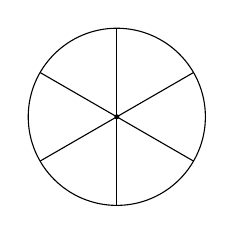
\begin{tikzpicture}[scale=0.75]
\draw (0,0) circle (1.5); \foreach \a in {30,90,...,330} \draw (0,0)--(\a:1.5); \fill (0,0) circle (1.2pt);
\end{tikzpicture}}
\Opts{$\dfrac12$}{$\dfrac16$}{$\dfrac14$}{$\dfrac13$}}
\QQ{33}{\Moslash{Uçburçakning tomonlari $9$, $10$ va $17$ ga teng. Bu uçburçakni eng katta balandligi atrofida $360^\circ$ aylantiriş natijasida jism hosil böldi. $\pi\approx3$ deb olinadi.}{A) $600$\par B) $945$\par C) $512$\par D) $567$\par E) $1462$\par F) $1512$}{Hosil bölgan jismning asosini (doiraviy halqasini) yuzini toping.}{Hosil bölgan jismning töla sirtidan asosining yuzining ayirmasini toping.}{Jismning hajmini toping.}}
\QQ{36}{Tenglamani yeçing:
\[\sqrt{1-x^2}=4x^3-3x\]
\AB{Tenglama neçta haqiqiy yeçimga ega?}{Tenglamaning haqiqiy ildizlari köpaytmasini toping.}}
\QQ{37}{Tenglamani yeçing:
\[5\sin^2x-\cos^2x+8\cos x=|\cos x|-1\]
\AB{Tenglama $\left[-\dfrac{5\pi}4;\,\dfrac{5\pi}4\right]$ oraliqda neçta ildizga ega?}{Tenglamaning $[0;\,6\pi]$ oraliqdagi yeçimlari yiğindisini toping.}}
\QQ{38}{$f(x)=ax^2+bx+c$ juft funksiya $y=4x-4$ töğri çiziqni bitta nuqtada kesadi va şu kesişiş nuqtasi $Ox$ öqida yotadi.
\AB{$\dfrac{a+b}c$ ning qiymatini toping.}{$f(-4)$ ning qiymatini toping.}}
\QQ{39}{Rasmda $y_1(x)$ yarim aylana, $y_2(x)$, $y_3(x)$ töğri çiziqlar tasvirlangan. $y_2(x)$ va $y_3(x)$ töğri çiziqlar özaro perpendikulyar. $y_1(x)$ yarim aylana $(0;0)$ va $(x_1;0)$ nuqtalardan ötadi. $y_2(x)$ töğri çiziq yarim aylana markazidan ötadi. $y_3(x)$ töğri çiziq $Ox$ öqini $(x_2;0)$ nuqtada kesib ötadi va $y_1(x)$ yarim aylanaga urinadi.
\qfig{\begin{tikzpicture}[scale=0.42,font=\small]
\draw[->] (-1.5,0)--(15,0) node[right] {$x$}; \draw[->] (0,-2.2)--(0,8.2) node[right] {$y$};
\draw (6,0) arc (0:180:3);
\draw (2.2,-2.26)--(5.0,5.66) node[right] {$y_2(x)=2\sqrt2x-6\sqrt2$};
\draw (-0.2,4.313)--(13.5,-0.531); \node[left] at (-0.2,4.313) {$y_3(x)$};
\draw ($(4,2.828)!0.45cm!(5,5.66)$) -- ($($(4,2.828)!0.45cm!(5,5.66)$)!1!-90:(4,2.828)$) -- ($(4,2.828)!0.45cm!(0,4.24)$);
\fill (0,0) circle (3pt); \fill (6,0) circle (3pt); \fill (12,0) circle (3pt);
\node[below left] at (0,0) {$(0;0)$}; \node[below] at (6,0) {$(x_1;0)$}; \node[above] at (12,0) {$(x_2;0)$};
\node at (1.8,1.6) {$y_1(x)$};
\end{tikzpicture}}
\AB{$x_1$ ni toping.}{$x_2$ ni toping.}}
\QQ{40}{$f(x)=a\cos(kx+\varphi)+b$ funksiyaning grafigi berilgan.
\qfig{\begin{tikzpicture}[x=1.05cm,y=0.42cm,font=\small]
\fill[qfill] plot[domain=1:3,samples=80,variable=\t] ({\t},{2-2*cos(\t*180)}) -- (3,0) -- (1,0) -- cycle;
\draw[->] (-0.2,0)--(5,0) node[right] {$x$}; \draw[->] (0,-0.5)--(0,5.2) node[above] {$y$};
\draw[thick,domain=0:4.7,samples=150,variable=\t] plot ({\t},{2-2*cos(\t*180)});
\draw[dashed] (0,4)--(3.6,4); \draw[dashed] (1,0)--(1,4); \draw[dashed] (3,0)--(3,4);
\node[left] at (0,4) {$4$}; \node[below left] at (0,0) {$O$};
\draw (2,0.12)--(2,-0.12) node[below] {$2\pi$}; \draw (4,0.12)--(4,-0.12) node[below] {$4\pi$};
\end{tikzpicture}}
\AB{$\dfrac{|a|+|b|}{|k|}$ ni toping.}{Böyalgan soha yuzini toping ($\pi\approx3$ deb olinadi).}}
\QQ{41}{$ABC$ uçburçakning $B$ uçidan $AC$ asosiga $BP$ va $BE$ kesmalar ötkazilgan bölib, bu kesmalar $GL$ örta çiziğini mos ravişda $H$ va $F$ nuqtalarda kesib ötadi. $BPE$ uçburçak yuzi $104$ ga teng. Agar $\dfrac{|AP|+|EC|}{AC}=\dfrac23$, $\dfrac{S_{BEC}}{S_{ABP}}=\dfrac49$ tengliklar örinli bölsa,
\qfig{\begin{tikzpicture}[scale=0.85,font=\small]
\coordinate (A) at (0,0); \coordinate (C) at (6,0); \coordinate (B) at (3.1,4.4); \coordinate (P) at (2.769,0); \coordinate (E) at (4.769,0);
\coordinate (G) at ($(A)!0.5!(B)$); \coordinate (L) at ($(C)!0.5!(B)$); \coordinate (H) at ($(B)!0.5!(P)$); \coordinate (F) at ($(B)!0.5!(E)$);
\draw (A)--(B)--(C)--cycle; \draw (B)--(P); \draw (B)--(E); \draw (G)--(L);
\node[below left] at (A) {$A$}; \node[above] at (B) {$B$}; \node[below right] at (C) {$C$}; \node[below] at (P) {$P$}; \node[below] at (E) {$E$};
\node[left] at (G) {$G$}; \node[right] at (L) {$L$}; \node[below left] at (H) {$H$}; \node[below right] at (F) {$F$};
\end{tikzpicture}}
\AB{$HGB$ uçburçak yuzini toping.}{$HLCP$ törtburçak yuzini toping.}}
\QQ{42}{Aylanaga $ABCD$ törtburçak taşqi çizilgan. $BC$ tomonning örtasidan $E$ nuqta, $AD$ tomonning örtasidan esa $F$ nuqta olingan. $EF$ töğri çiziq hamda $AC$ va $BD$ diagonallar $P$ nuqtada kesişadi va $PF=3EP$. Agar $AB=6$, $AC=2\sqrt{13}$ bölsa,
\AB{$\cos(\angle ADC)$ ni toping.}{Aylana radiusini toping.}}
\QQ{43}{Muntazam oltiburçakning içidan $K$ nuqta olingan va undan $B$, $D$, $F$ uçlarigaça bölgan masofalar $11$, $10$, $5$ ga teng bölsa,
\qfig{\begin{tikzpicture}[scale=1,font=\small]
\coordinate (A) at (-2.674,0.000); \coordinate (B) at (-1.337,2.316); \coordinate (C) at (1.337,2.316); \coordinate (D) at (2.674,0.000); \coordinate (E) at (1.337,-2.316); \coordinate (F) at (-1.337,-2.316); \coordinate (K) at (-0.344,-1.060);
\draw (A)--(B)--(C)--(D)--(E)--(F)--cycle; \draw (B)--(K)--(D); \draw (F)--(K)--(A); \fill (K) circle (1.3pt);
\node[left] at (A) {$A$}; \node[above left] at (B) {$B$}; \node[above right] at (C) {$C$}; \node[right] at (D) {$D$}; \node[below right] at (E) {$E$}; \node[below left] at (F) {$F$}; \node[below right] at (K) {$K$};
\node[right] at ($(B)!0.5!(K)$) {$11$}; \node[above] at ($(D)!0.5!(K)$) {$10$}; \node[right] at ($(F)!0.5!(K)$) {$5$};
\end{tikzpicture}}
\AB{Muntazam oltiburçak tomonini toping.}{$AK$ kesma uzunligini toping.}}
\QQ{44}{Asosining tomonlari $3$ va $4$ ga teng bölgan muntazam uçburçakli kesik piramidaga şar içki çizilgan.
\AB{Şar radiusini toping.}{Kesik piramida hajmini toping.}}
\QQ{45}{Tomoni $6$ m ga teng bölgan $ABCD$ kvadrat berilgan. Kvadrat içidan olingan ixtiyoriy $O$ nuqtadan $AB$ tomongaça bölgan eng qisqa masofa $2$ m ga, $BC$ tomongaça bölgan eng qisqa masofa $3$ m ga teng.
\AB{$O$ nuqta orqali ötkazilgan töğri çiziq kvadratdan qanday eng katta yuzali (m$^2$) uçburçak ajratadi?}{$O$ nuqta orqali töğri çiziq ötkazilganda hosil böladigan şakllarning yuzalari $S_1$ va $S_2$ ga teng bölsa, $|S_1-S_2|$ ning eng katta (sm$^2$) qiymatini toping.}}
\Javoblar{B B A B B C D B A A D B C D A B B C A C C D A B B B B A B A A A D B F}{%
\OK{36}{$3$}{$\dfrac14$}\OK{37}{$2$}{$18\pi$}\OK{38}{$-1$}{$30$}\OK{39}{$6$}{$12$}\OK{40}{$4$}{$12$}%
\OK{41}{$36$}{$126$}\OK{42}{$\dfrac45$}{$3$}\OK{43}{$\sqrt{41+8\sqrt{13}}$}{$8$}\OK{44}{$1$}{$\dfrac{37\sqrt3}6$}\OK{45}{$13{,}5$}{$120\,000$}}
